\section{Numerical Algorithm}\label{eq:algorithm}
\subsection{Spatial Discretization}\label{Sec:Spatial}
The spatial discretization and adaptive mesh refinement methodology remains unchanged from Paper V.
We now summarize some of the key points here before describing the new temporal integrator in the next section.
We recommend the reader review Section 3 of Paper V for further details.

We shall refer to local atmospheric flows in two and three dimensions as problems in ``planar'' geometry, and full-star flows
in three dimensions as problems in ``spherical'' geometry.
The solution in both cases consists of the Cartesian grid solution
and the one-dimensional base state solution.
Figure \ref{Fig:BaseGrid} illustrates the relationship between the base state and the Cartesian grid state for both planar and spherical geometries in the presence of spatially adaptive grids. 
%%%%%%%%%%%%%%%%%%%%%%%%%%%%%%%%%
\begin{figure}[tb]
\centering
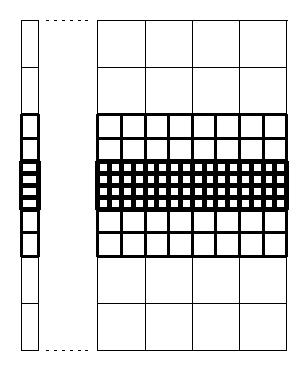
\includegraphics[height=2.0in]{./figs/base_grid} \hspace{0.5in}
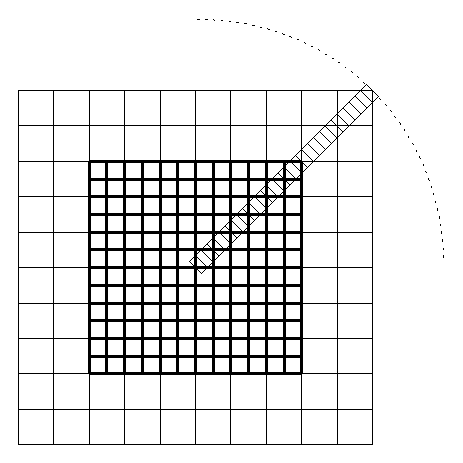
\includegraphics[height=2.0in]{./figs/base_spherical}
\caption{\label{Fig:BaseGrid}  
(Left) For multi-level problems in planar geometry, we force a direct alignment
between the base state cell centers and the Cartesian grid cell centers by 
allowing the radial base state spacing to change with space and time.
(Right) For multi-level problems in spherical geometry, since there is no direct alignment
between the base state cell centers and the Cartesian grid cell centers, we choose to fix
the radial base state spacing across levels. Reprinted from Paper V \citep{MAESTRO_V}. }
\end{figure}
%%%%%%%%%%%%%%%%%%%%%%%%%%%%%%%%%
One of the key numerical modules is the ``lateral average'', which computes the average over a 
layer of constant radius of a Cartesian grid variable and stores the result in a one-dimensional base state array.
In planar geometries, this is a straightforward arithmetic average of values in cells at
a particular height since the base state cell centers are in alignment
with the Cartesian grid cell centers.
However for spherical problems, the procedure is much more complicated.
In Section 4 of Paper V, we describe how there is a finite, easily computable set of radii that any 
there-dimensional Cartesian cell-center can map to.  
Specifically, for every three-dimensional Cartesian cell, there exists an integer $m$ such that the distance
from the cell center to the center of the star is given by 
\begin{equation}
\hat{r}_m=\Delta x\sqrt{0.75+2m}.\label{eqn:radii}
\end{equation}
%%%%%%%%%%%%%%%%%%%%%%%%%%%%%%%%%
\begin{figure}[tb]
\centering
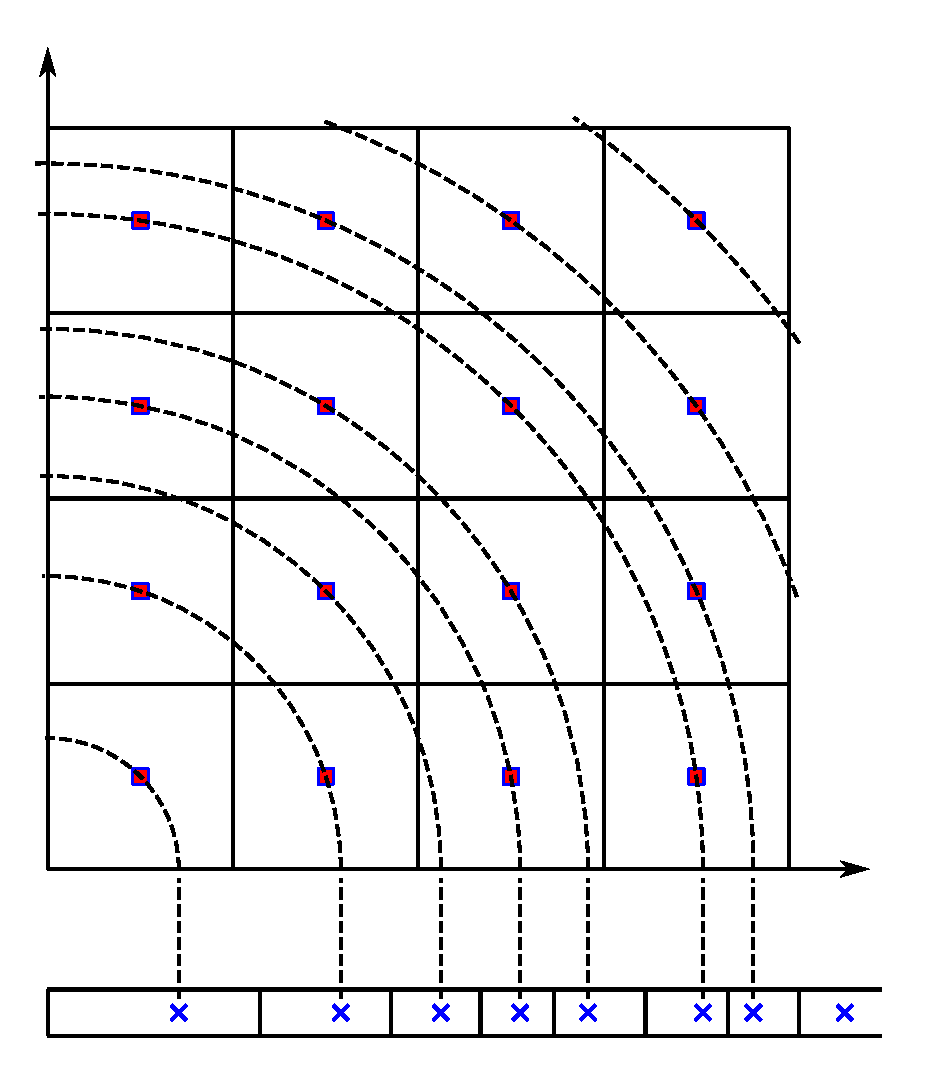
\includegraphics[height=2.5in]{./figs/base_spherical_new}
\caption{\label{Fig:NewBaseGrid}  
A direct mapping between the base state cell centers (red squares) and the Cartesian grid cell centers (blue crosses) 
is enforced by computing the average of the grid cell centers that share the same radial distance from 
the center of the star.}
\end{figure}
%%%%%%%%%%%%%%%%%%%%%%%%%%%%%%%%%
Figure \ref{Fig:NewBaseGrid} is a two-dimensional illustration 
(two dimensions is chosen in the figure for ease of exposition; this mapping is only used for three-dimensional spherical stars) 
of the relationship between the Cartesian grid state and the one-dimensional base state array.
We compute the lateral average by first summing the values in all the cells associated with each radius,
dividing by the number of contributing cells to obtain the arithmetic average, and then use quadratic interpolation to map this data onto a one-dimensional base state.
Previously, for spherical problems MAESTRO only allowed for a base state with constant $\Delta r$ (typically equal to $\Delta x/5$).

The companion ``fill'' module maps a base state array onto the full Cartesian grid state.
For planar problems, direct injection can be used due to the perfect alignment of the base state and Cartesian grid state.
For spherical problems, quadratic interpolation of the base state is used to assign values to each Cartesian cell center.

In this paper we explore a new option to retain an irregularly-spaced base state to eliminate mapping errors from the ``fill'' module.
For the lateral average, as before we first sum the values in all the cells associated with each radius and divide
by the number of contributing cells to obtain the arithmetic average.  However we do not interpolate this onto a uniformly spaced
base state and retain the use of this irregularly-spaced base state.
The advantage with this approach is that the fill module does not require any interpolation.
A potential benefit to eliminating the mapping error is to consider a spherical star in hydrostatic equilibrium at rest.
In the absence of reactions, the star should remain at rest.
The buoyancy forcing term in the momentum equation contains $\rho-\rho_0$.  With the original scheme, interpolation errors 
in computing $\rho_0$ by averaging would cause artificial acceleration in the velocity field due to the interpolation error 
from the Cartesian grid to and from the radial base state.  By retaining the radial base state as an irregularly spaced array, 
\replaced{the effects due to interpolation error are nearly eliminated, but not completely eliminated since there are still machine precision 
effects resulting from averaging a large number of numerical values.}
{the truncation error in the mapping scheme is completely eliminated.  The only source of error is due to machine precision effects resulting 
from averaging a large number of values, which is not significant over the course of any simulation.}
We note that $\Delta r$ decreases as the base state moves further from the center of the star, 
which results in far more total cells in the irregularly-spaced array than the previous uniformly-spaced array. 

\subsection{Temporal Integration Scheme}\label{Sec:Temporal Integration Scheme}
We now describe the new temporal integration scheme, noting that it can be used for the original base state mapping 
(with uniform base state grid spacing) as well as the new irregularly spaced base state mapping.
Previously we adopted an approach where we split the velocity into a base state component, $w_0(r,t)$, 
and a local velocity $\Ubt(\xb,t)$, so that
\begin{equation}
\Ub = \Ubt(\xb,t) + w_0(r,t)\eb_r, \label{eq:velsplit}
\end{equation}
where $\eb_r$ is the normal vector in the outward radial direction.
We used $w_0$ to provide an estimate of the base state density evolution over a time step.
This resulted in some unnecessary complications to the temporal integration scheme including
base state advection modules for density, enthalpy, and velocity, as well as more 
cumbersome split velocity dynamics evolution equations.
Our new temporal integration scheme uses full velocities for scalar and velocity advection,
and only uses the above splitting to satisfy the velocity divergence constraint due to boundary considerations
at the edge of the star.
This results in a much simpler numerical scheme than the one from Paper V 
since we use the velocity directly rather than more complex terms involving the perturbational velocity.
Additionally, the new scheme uses a simpler predictor-corrector approach to the base state density and pressure that no 
longer requires evolution equations and numerical discretizations to update the base state, greatly 
simplifying the algorithm while retaining the same overall second-order accuracy in time.

At the beginning of each time step we have the cell-centered Cartesian grid state,
$(\Ub,\rho X_k,\rho h)^n$, and nodal Cartesian grid state, $\pi^{n-\myhalf}$, and base state $(\rho_0,p_0)^n$.
At any time, the associated density, composition, and enthalpy can be trivially computed using, e.g.,
\begin{equation}
\rho^n = \sum_k(\rho X_k)^n, \quad
X_k^n = (\rho X_k)^n / \rho^n, \quad
h^n = (\rho h)^n / \rho^n.
\end{equation}
Temperature is computed using the equation of state\footnote{As described in Paper V, for planar problems we compute temperature using $h$ instead of $p_0$, since we have successfully developed volume discrepancy schemes to effectively couple the enthalpy to the rest of the solution; see \cite{XRB_I}.  We are still exploring this option for spherical stars.}, e.g.,
$T = T(\rho,p_0,X_k)$, where $p_0$ has been mapped to the Cartesian grid using the fill module,
and ($\gammaonebar,\beta_0)$ are similarly computed from $(\rho,p_0,X_k)$;
see Appendix A of Paper I and Appendix C of Paper III for details on how $\beta_0$ is computed.

The overall flow of the algorithm begins with a second-order Strang splitting approach to integrate the advection-reaction system for 
the thermodynamic variables $(\rho X_k, \rho h)$, followed by a second-order projection methodology to integrate the velocities subject to a divergence constraint.  Within the thermodynamic variable update we use a predictor-corrector approach to achieve second-order accuracy in time.
To summarize:
\begin{itemize}
\item In {\bf Step 1} we react the thermodynamic variables over the first $\Delta t/2$ interval.
\item In {\bf Steps 2--4} we advect the thermodynamic variables over $\Delta t$.  Specifically, we compute an estimate for the expansion term, $S$, compute face-centered, time-centered velocities that satisfy the divergence constraint, and then advect the thermodynamic variables.
\item In {\bf Step 5} we react the thermodynamic variables over the second $\Delta t/2$ interval\footnote{After this step we could skip to the velocity advance in {\bf Steps 10--11}, however the overall scheme would be only first-order in time, so {\bf Steps 6-9} can be thought of as a trapezoidal corrector step.}.
\item In {\bf Steps 6--8} we redo the advection in {\bf Steps 2--4} but are able to use the trapezoidal rule to time-center certain quantities such as $S$, $\rho_0$, etc.
\item In {\bf Step 9} we redo the reactions from {\bf Step 5} beginning with the improved results from {\bf Steps 6--8}.
\item In {\bf Steps 10--11} we advect the velocity, and then project these velocities so they satisfy the divergence constraint while updating $\pi$.
\end{itemize}

There are a few key numerical modules we use in each time step.
\begin{itemize}
\item {\bf Average}$[\phi]\rightarrow[\overline\phi]$ computes the lateral average of a quantity over a layer at constant radius $r$, as described above in Section \ref{Sec:Spatial}.
\item {\bf Enforce HSE}$[\rho_0]\rightarrow[p_0]$ computes the base state pressure, $p_0$, from a base state density, $\rho_0$ by integrating the hydrostatic equilibrium condition in one dimension. 
This follows equation (A10) in Paper V, noting that for the irregularly spaced base state case, $\Delta r$ is not constant, where $\Delta r_{j+1/2} = r_{j+1} - r_j$ for cell face with index $j+1/2$.  
The base state pressure remains equal to a constant value at the location of a prescribed cutoff density outward for the entire simulation.
\item {\bf React State}$[(\rho X_k)^{\rm in},(\rho h)^{\rm in},p_0]\rightarrow[(\rho X_k)^{\rm out},(\rho h)^{\rm out},(\rho\dot\omega),(\rho\Hnuc)]$ 
uses 
\added{the multistep variable-coefficient Adams-Moulton and Backward Differentiation Formula (BDF) methods in the}
VODE \citep{vode} 
\added{package}
to integrate the species and enthalpy due to reactions over $\Delta t/2$ by solving
\begin{equation}
\frac{dX_k}{dt} = \dot\omega_k(\rho,X_k,T); \qquad
\frac{dT}{dt} = \frac{1}{c_p}\left(-\sum_k\xi_k\dot\omega_k + H_{\rm nuc})\right)
\end{equation}
The inputs are the species, enthalpy, and base state pressure, and the outputs are the species, enthalpy, reaction rates, and nuclear energy generation rate.
See Paper III for details.
\end{itemize}
Each time step is constrained by the standard advective CFL condition,
\begin{equation}
\Delta t = \sigma^{\rm CFL} \min_i(\Delta x / U_i),
\end{equation}
where for our simulations we typically use $\sigma^{\rm CFL}\sim 0.7$ and the minimum is taken over all spatial directions over all cells.
\replaced{There are additional constraints on the time step that are typically much less restrictive than the advective CFL including
the acceleration due to the buoyancy force (sometimes in effect when the velocity is approximately zero at the start of some simulations) 
and the local magnitude of the divergence constraint (to prevent too much mass evacuation from a cell in a time step);}
{For simulations that are initialized with zero velocity, we use the buoyancy force in the momentum equation to give a proper time scale
to start the simulation;} see Section 3.4 in Paper III for details.

In stratified low Mach number models, due to the extreme variation in density, the velocity can become very large in low density regions at the edge of the star.
These large velocities can severely affect the time step, so
throughout Papers II-V, we have employed two techniques to help control these dynamics without significantly 
affecting the dynamics in the convective region.
First, we use a cutoff density technique, where we hold the density constant outside a specified radius (typically near where the density is $\sim$4 orders of magnitude smaller than the largest densities in the simulation).
Second, we employ a sponge technique where we artificially damp the velocities near and beyond the cutoff region.
For more details, refer to Paper V and the previous references cited within.

Beginning with $(\Ub,\rho X_k,\rho h)^n$, $\pi^{n-\myhalf}$, and $(\rho_0,p_0)^n$,
the temporal integration scheme contains the following steps:
\begin{description}

%--------------------------------------------------------------------------
% STEP 1
%--------------------------------------------------------------------------
\item[Step 1] {\em React the thermodynamic variables over the first $\Delta t / 2$ interval.}

Call {\bf React State}$[(\rho X_k)^n, (\rho h)^n, p_0^n] \rightarrow [(\rho X_k)^{(1)}, (\rho h)^{(1)}, (\rho \omegadot_k)^{(1)}, (\rho \Hnuc)^{(1)}]$.

%--------------------------------------------------------------------------
% STEP 2
%--------------------------------------------------------------------------

\item[Step 2] {\em Compute the time-centered expansion term, $S^{\nph,\star}$.}

We compute an estimate for the time-centered expansion term in the velocity
divergence constraint.  Following \citet{Bell:2004}, we extrapolate
to the half-time using $S$ at the previous and current
time steps,
\begin{equation}
S^{\nph,\star} = S^n + \frac{\dt^n}{2} \left(\frac{S^n - S^{n-1}}{\dt^{n-1}}\right).
\end{equation}
Note that in the first time step we average $S^0$ and $S^1$ from the
initialization step.

%--------------------------------------------------------------------------
% STEP 3
%--------------------------------------------------------------------------
\item[Step 3] {\em Construct a face-centered, time-centered advective velocity, $\uadvone$.}

The construction of face-centered time-centered states used to discretize the
advection terms for velocity, species, and enthalpy, are performed using
a standard multidimensional corner transport upwind approach
\citep{colella1990multidimensional,saltzman1994unsplit} with the piecewise-parabolic method (PPM)
one-dimensional tracing \citep{colella1984piecewise}.  The full details of this
Godunov advection approach for all steps in this algorithm are described 
in Appendix A of \cite{XRB_III}.
Here we use equation (\ref{eq:momentum}) to compute face-centered, time-centered velocities, $\uadvonedag$.
The $\dagger$ superscript refers to the fact that the predicted velocity field does not satisfy the divergence constraint,
\begin{equation}
\nabla \cdot \left(\beta_0^n \uadvone\right) = \beta_0^n \left[S^{\nph,\star} - \frac{1}{\gammaonebar^np_0^n}\left(\frac{\partial p_0}{\partial t}\right)^{n-\myhalf} \right].\label{eq:div1}
\end{equation}
 We project $\uadvonedag$ onto the space of velocities that satisfy the constraint to obtain $\uadvone$.
Each projection step in the algorithm involves the solution of a variable-coefficient Poisson solve using multigrid.
Note that we still employ velocity-splitting as described by equation (\ref{eq:velsplit}) for this step 
in order to enforce the appropriate behavior of the system near the edge of the star as determined by the cutoff density.
The details of this ``MAC'' projection are provided in Appendix \ref{Sec:Projection}.

%--------------------------------------------------------------------------
% STEP 4
%--------------------------------------------------------------------------
\item[Step 4] {\em Advect the thermodynamic variables over a time interval of $\dt.$}

\begin{enumerate}
\renewcommand{\theenumi}{{\bf \Alph{enumi}}}

\item Update $(\rho X_k)$ using a discretized version of
%
\begin{equation}
\frac{\partial(\rho X_k)}{\partial t} = -\nabla\cdot(\rho X_k\Ub),
\end{equation}
%
where the reaction terms have been omitted since they were already 
accounted for in {\bf React State}.  The update consists of two steps:

\begin{enumerate}
\renewcommand{\labelenumii}{{\bf \roman{enumii}}.}

\item Compute the face-centered, time-centered species, $(\rho X_k)^{\nph,\pred,\star}$,
  for the conservative update of $(\rho X_k)^{(1)}$ using a Godunov approach \citep{XRB_III}.
  As described in Paper V, for robust numerical slope limiting we predict 
  $\rho'^n=\rho^n-\rho_0^n$ and $X_k^n$ to faces
  and here we spatially interpolate $\rho_0^n$ to faces to assemble the fluxes.

\item Evolve $(\rho X_k)^{(1)} \rightarrow (\rho X_k)^{(2),\star}$ using
\begin{equation}
(\rho X_k)^{(2),\star} = (\rho X_k)^{(1)}
  - \dt \left\{ \nabla \cdot \left[ \uadvone (\rho X_k)^{\nph,\pred,\star} \right] \right\},
\end{equation}

\end{enumerate}

\item Update $\rho_0$ by calling {\bf Average}$[\rho^{(2),\star}]\rightarrow[\rho_0^{n+1,\star}]$.

\item Update $p_0$ by calling {\bf Enforce HSE}$[\rho_0^{n+1,\star}] \rightarrow [p_0^{n+1,\star}]$.

\item Update the enthalpy using a discretized version of equation
%
\begin{equation}
\frac{\partial(\rho h)}{\partial t} = -\nabla\cdot(\rho h\Ub) + \frac{Dp_0}{Dt} + \rho\Hnuc,
\end{equation}
%
again omitting the reaction terms since we already accounted for
them in {\bf React State}.  This equation takes the form:
\begin{equation}
\frac{\partial (\rho h)}{\partial t}  = - \nabla \cdot (\rho h\Ub) + \frac{\partial p_0}{\partial t} + (\Ub \cdot \eb_r) \frac{\partial p_0}{\partial r}.
\end{equation}
For spherical geometry, we solve the analytically equivalent form,
\begin{equation}
\frac{\partial (\rho h)}{\partial t}  = - \nabla \cdot (\rho h\Ub) + \frac{\partial p_0}{\partial t} + \nabla \cdot (\Ub p_0) - p_0 \nabla \cdot \Ub.
\end{equation}
The update consists of two steps:

\begin{enumerate}
\renewcommand{\labelenumii}{{\bf \roman{enumii}}.}

\item Compute the face-centered, time-centered enthalpy, $(\rho h)^{\nph,\pred,\star},$
  for the conservative update of $(\rho h)^{(1)}$ using using a Godunov approach \citep{XRB_III}.
  As described in Paper V, for robust numerical slope limiting 
  we predict $(\rho h)'^n=(\rho h)^n-(\rho h)_0^n$ to faces,
  where $(\rho h)_0^n$ is obtained by calling {\bf Average}$[(\rho h)^n]\rightarrow[(\rho h)_0^n]$,
  and here we spatially interpolate $(\rho h)_0^n$ to faces to assemble the fluxes.

\item Evolve $(\rho h)^{(1)} \rightarrow (\rho h)^{(2),\star}$ using
\begin{equation}
(\rho h)^{(2),\star}
= (\rho h)^{(1)} - \dt \left\{ \nabla \cdot \left[ \uadvone (\rho h)^{\nph,\pred,\star} \right] \right\} + \Delta t\frac{Dp_0}{Dt}
\end{equation}
where here
\begin{equation}
\frac{Dp_0}{Dt} =
\begin{cases}
\frac{p_0^{n+1,*} - p_0^n}{\Delta t} + \left(\uadvone \cdot \eb_r\right) \left(\frac{\partial p_0}{\partial r} \right)^{n}& {\rm (planar)} \\
\frac{p_0^{n+1,*} - p_0^n}{\Delta t} + \left[ \nabla \cdot \left (\uadvone p_0^{\nph} \right ) - p_0^{\nph} \nabla \cdot \uadvone \right]& {\rm (spherical)}
\end{cases}
,
\end{equation}
and $p_0^\nph = (p_0^n+p_0^{n+1,*})/2$.
\end{enumerate}
\end{enumerate}

%--------------------------------------------------------------------------
% STEP 5
%--------------------------------------------------------------------------
\item[Step 5] {\em React the thermodynamic variables over the second $\Delta t / 2$ interval.}

Call {\bf React State}$[ (\rho X_k)^{(2),\star}, (\rho h)^{(2),\star}, p_0^{n+1,\star}] 
\rightarrow 
[ (\rho X_k)^{n+1,\star}, (\rho h)^{n+1,\star}, (\rho \omegadot_k)^{n+1,\star}, (\rho \Hnuc)^{n+1,\star} ].$

%--------------------------------------------------------------------------
% STEP 6
%--------------------------------------------------------------------------
\item[Step 6] {\em Compute the time-centered expansion term, $S^{\nph,\star}$.}

First, compute $S^{n+1,\star}$ with
\begin{equation}
S^{n+1,\star} =  \left(-\sigma  \sum_k  \xi_k  \omegadot_k  + \frac{1}{\rho p_\rho} \sum_k p_{X_k}  {\omegadot}_k + \sigma \Hnuc\right)^{n+1,\star}.
\end{equation}
  Then, define
\begin{equation}
 S^{\nph} = \frac{S^n + S^{n+1,\star}}{2},
\end{equation}

%--------------------------------------------------------------------------
% STEP 7
%--------------------------------------------------------------------------
\item[Step 7] {\em Construct a face-centered, time-centered advective velocity, $\uadvtwo$.}

The procedure to construct $\uadvtwodag$ is identical to the Godunov procedure
for computing $\uadvonedag$ in {\bf Step 3}, but uses
the updated value $S^{\nph}$ rather than $S^{\nph,\star}$.
The $\dagger$ superscript refers to the fact that the predicted velocity field does not satisfy the divergence constraint,
\begin{equation}
\nabla \cdot \left(\beta_0^{\nph} \uadvtwo\right) =
\beta_0^{\nph} \left[S^{\nph} - \frac{1}{\gammaonebar^{\nph}p_0^{\nph}}\left(\frac{\partial p_0}{\partial t}\right)^{\nph}\right],\label{eq:div2}
\end{equation}
with
\begin{equation}
\beta_0^{\nph} = \frac{ \beta_0^n +  \beta_0^{n+1,\star} }{2}, \quad
\gammaonebar^{\nph} = \frac{ \gammaonebar^n +  \gammaonebar^{n+1,\star} }{2}.
\qquad
\end{equation}
we project $\uadvtwodag$ onto the space of velocities that satisfy the constraint to obtain $\uadvtwo$ using a MAC projection (see Appendix \ref{Sec:Projection}).

%--------------------------------------------------------------------------
% STEP 8
%--------------------------------------------------------------------------
\item[Step 8] {\em Advect the thermodynamic variables over a time interval of $\dt.$}

\begin{enumerate}
\renewcommand{\theenumi}{{\bf \Alph{enumi}}}

\item Update $(\rho X_k)$.  This step is identical to {\bf Step 4A} except we use
  the updated values $\uadvtwo$ and $\rho_0^{n+1,\star}$ rather than
  $\uadvone$ and $\rho_0^n$.  In particular:

\begin{enumerate}
\renewcommand{\labelenumii}{{\bf \roman{enumii}}.}

\item Compute the face-centered, time-centered species, $(\rho X_k)^{\nph,\pred}$,
  for the conservative update of $(\rho X_k)^{(1)}$ using a Godunov approach \citep{XRB_III}.
  Again, we predict $\rho'^n=\rho^n-\rho_0^n$ and $X_k^n$ to faces
  but here we spatially interpolate $(\rho_0^n+\rho_0^{n+1,*})/2$ to faces to assemble the fluxes.


\item Evolve $(\rho X_k)^{(1)} \rightarrow (\rho X_k)^{(2)}$ using
\begin{equation}
(\rho X_k)^{(2)} = (\rho X_k)^{(1)}
- \dt \left\{ \nabla \cdot \left[\uadvtwo (\rho X_k)^{\nph,\pred} \right] \right\},
\end{equation}

\end{enumerate}

\item Update $\rho_0$ by calling {\bf Average}$[\rho^{(2)}]\rightarrow[\rho_0^{n+1}]$.

\item Update $p_0$ by calling {\bf Enforce HSE}$[\rho_0^{n+1}] \rightarrow [p_0^{n+1}]$.

\item Update the enthalpy.  This step is identical to {\bf Step 4D} except we use
  the updated values $\uadvtwo$, $\rho_0^{n+1}$, $(\rho h)_0^{n+1}$, and $p_0^{n+1}$
  rather than
  $\uadvone, \rho_0^n$, $(\rho h)_0^n$, and $p_0^n$.
  In particular:

\begin{enumerate}
\renewcommand{\labelenumii}{{\bf \roman{enumii}}.}

\item Compute the face-centered, time-centered enthalpy, $(\rho h)^{\nph,\pred},$
  for the conservative update of $(\rho h)^{(1)}$ using a Godunov approach \citep{XRB_III}.
  Again, we predict $(\rho h)'^n=(\rho h)^n-(\rho h)_0^n$ to faces
  but here we spatially interpolate $[(\rho h)_0^n)+(\rho h)_0^{n+1,*}]/2$ to faces to assemble the fluxes.

\item Evolve $(\rho h)^{(1)} \rightarrow (\rho h)^{(2)}$.
\begin{equation}
(\rho h)^{(2)}
= (\rho h)^{(1)} - \dt \left\{ \nabla \cdot \left[ \uadvtwo (\rho h)^{\nph,\pred} \right] \right\} + \Delta t\frac{Dp_0}{Dt}
\end{equation}
where here
\begin{equation}
\frac{Dp_0}{Dt} =
\begin{cases}
\frac{p_0^{n+1} - p_0^n}{\Delta t} + \left(\uadvtwo \cdot \eb_r\right) \left(\frac{\partial p_0}{\partial r} \right)^{n}& {\rm (planar)} \\
\frac{p_0^{n+1} - p_0^n}{\Delta t} + \left[ \nabla \cdot \left (\uadvtwo p_0^{\nph} \right ) - p_0^{\nph} \nabla \cdot \uadvtwo \right]& {\rm (spherical)}
\end{cases}
,
\end{equation}
and $p_0^\nph = (p_0^n+p_0^{n+1})/2$.
\end{enumerate}
\end{enumerate}

%--------------------------------------------------------------------------
% STEP 9
%--------------------------------------------------------------------------
\item[Step 9] {\em React the thermodynamic variables over the second $\Delta t / 2$ interval.}

Call {\bf React State}$[(\rho X_k)^{(2)},(\rho h)^{(2)}, p_0^{n+1}] \rightarrow [(\rho X_k)^{n+1}, (\rho h)^{n+1}, (\rho \omegadot_k)^{n+1}, (\rho \Hnuc)^{n+1}].$

%--------------------------------------------------------------------------
% STEP 10
%--------------------------------------------------------------------------
\item[Step 10] {\em Define the new-time expansion term, $S^{n+1}$.}

\begin{enumerate}
\renewcommand{\theenumi}{{\bf \Alph{enumi}}}
\item Define
\begin{equation}
  S^{n+1} =  \left(-\sigma  \sum_k  \xi_k \omegadot_k  + \sigma \Hnuc +
  \frac{1}{\rho p_\rho} \sum_k p_{X_k}  \omegadot_k\right)^{n+1}.
\end{equation}

\end{enumerate}


%--------------------------------------------------------------------------
% STEP 11
%--------------------------------------------------------------------------
\item[Step 11] {\em Update the velocity}.

First, we compute the face-centered, time-centered velocities, $\Ub^{\nph,\pred}$
using a Godunov approach \citep{XRB_III}. Then, we update
the velocity field $\Ub^n$ to $\Ub^{n+1,\dagger}$ by discretizing
equation (\ref{eq:momentum}) as
\begin{equation}
\Ub^{n+1,\dagger}
= \Ub^n - \dt \left[\uadvtwo \cdot \nabla \Ub^{\nph,\pred} \right]
 - \dt \left[ \frac{\beta_0^\nph}{\rho^\nph} \nabla \left( \frac{\pi^\nmh}{\beta_0^\nmh} \right) + \frac{\left(\rho^\nph-\rho_0^\nph\right)}{\rho^\nph} g^{\nph} \eb_r \right],
\end{equation}
where
\begin{equation}
\rho^\nph = \frac{\rho^n + \rho^{n+1}}{2}, \qquad \rho_0^\nph = \frac{\rho_0^n + \rho_0^{n+1}}{2}.
\end{equation}
Again, the $\dagger$ superscript refers
to the fact that the updated velocity does not satisfy the divergence constraint,
\begin{equation}
\nabla \cdot \left(\beta_0^{n+1} \Ub^{n+1} \right) = \beta_0^{n+1} \left[ S^{n+1} - \frac{1}{\gammaonebar^{n+1}p_0^{n+1}}\left(\frac{\partial p_0}{\partial t}\right)^{\nph}\right].\label{eq:div3}
\end{equation}
We use an approximate projection to project $\Ub^{n+1,\dagger}$ onto the space of velocities that satisfy the constraint to obtain $\Ub^{n+1}$ using a ``nodal'' projection.
This projection necessarily differs from the MAC projection used in
{\bf Step 3} and {\bf Step 7} because the velocities in those steps are defined
on faces and $\Ub^{n+1}$ is defined at cell centers, requiring different divergence
and gradient operators.
Furthermore, as part of the nodal projection, we also define a nodal new-time perturbational pressure, $\pi^\nph$.
Refer to Appendix \ref{Sec:Projection} for more details.

\end{description}
This completes one step of the algorithm.

To initialize the simulation we use the same procedure described in Paper III.
At the beginning of each simulation, we define $(\Ub,\rho X_k,\rho h)$.
We set initial values for $\Ub, \rho X_k$, and $\rho h$ and perform a sequence of projections 
(to ensure the velocity field satisfies the divergence constraint) 
followed by a small number of steps of the temporal advancement scheme to iteratively 
find initial values for $\pi^{n-\myhalf}$ and $S^0$ and $S^1$ for use in the first time step.

Our approach to adaptive mesh refinement is algorithmically the same as the treatment described 
in Section 5 of Paper V; we refer the reader there for details.
MAESTROeX supports refinement ratios of 2 between levels.
We note that for spherical problems, AMR is only available for the case of a uniformly-spaced base state.
